\documentclass[12pt]{article}
\usepackage{latexsym}
\usepackage{fancyhdr}
\usepackage{amssymb,amsmath,amsthm}
\usepackage[pdftex]{graphicx}
\usepackage{pdfpages}
\usepackage[margin=1in]{geometry}


% Create answer counter to keep track of seperate responses
\newcounter{AnswerCounter}
\newcounter{SubAnswerCounter}
\setcounter{AnswerCounter}{1}
\setcounter{SubAnswerCounter}{1}

% Create answer environment which uses counter
\newenvironment{answer}[0]{
  \setcounter{SubAnswerCounter}{1}
  \bigskip
  \textbf{Solution \arabic{AnswerCounter}}
  \\
  \begin{small}
}{
  \end{small}
  \stepcounter{AnswerCounter}
}

\newenvironment{subanswer}[0]{
  (\alph{SubAnswerCounter})
}{
 \bigskip
  \stepcounter{SubAnswerCounter}
}

% Allows easy use of vectors
\newcommand{\vect}[1]{\vec{\boldsymbol{#1}}}

% Setting up the title
\title{Mathematics 131 \\
Topology I}
\author{
        Luis Antonio Perez \\
        HUID: 70871564 \\
        Harvard College \\
        \href{mailto:luisperez@college.harvard.edu}{luisperez@college}
}
\date{\today}

% Custom Header information on each page
\pagestyle{fancy}
\lhead{HUID: 70871564}
\rhead{Perez - \thepage}
\renewcommand{\headrulewidth}{0.1pt}
\renewcommand{\footrulewidth}{0.1pt}

% Title page is page 0
\setcounter{page}{0}

\begin{document}
\begin{answer}[Page 335, \#5]
We let $A$ be a subspace of $\mathbb{R}^n$ and $h: (A, a_0) \to (Y, y_0)$. We show that if $h$ is extendable to a continuous map of $\mathbb{R}^n$ into $Y$, then $h_*$ is the trivial homeomorphism.
\begin{proof}
Let $\bar{h} (\mathbb{R}^n, a_0) \to (Y, y_0)$ be the extension of $h$. Now consider any loop $f$ in $A$ based at $a_0$. We first show that for any such loop, the path $h \circ f$ is nullhomotopic. We can define the following homotopy $F: A \times [0,1] \to Y$:
$$
F(a, t) = \bar{h}((1-t)f(a) + a_0t)
$$
We immediately have that $F(a,0) = \bar{h}(f(a)) = (h \circ f)(a)$ and $F(a,1) = \hbar{a_0} = h(a_0) = y_0$ (by the fact that $\bar{h}$ is an extension of $h$,and that $F$ is continuous by the continuity of $\bar{h}$ defined on all of $\mathbb{R}^n$. Therefore, $h \circ f$ is nullhomotopic. The note:
$$
h_*([f]) = [h \circ f] = [e_{y_0}]
$$
by the fact that $h \circ f$ is nullhomotopic.
\end{proof}
\end{answer}

\begin{answer}[Page 341, \#3]
We let $p: E \to B$ be a covering map, with $B$ connected. We now show that if $p^{-1}(b_0)$ has $k$ elements for some $b_0 \in B$, then $p^{-1}(b)$ has $k$ elements for every $b \in B$, and is called a $k$-fold covering of $B$.
\begin{proof}
Let us consider the set $C_k = \{ b \in B \mid p^{-1}(b) \text{ has $k$ elements} \}$. We will show that $C_k = B$ (ie, is the entire space. To do this, first note that the only sets that are both open and closed in $B$ (due to connectivity) are $B$ and $\emptyset$. Therefore, if we can show that $C_k$ is both open and closed and non-empty, then the implication is that $C_k = B$.
\begin{itemize}
\item It is clear that $C_k \neq \emptyset$ since, by the problem statement, we have $b_0 \in C_k$.
\item Since $p$ is a covering map, then every point $b \in B$ has an open neighborhood $U_b$ that is evenly covered. Therefore, this implies that $p^{-1}(b)$ can be written as the union of disjoint open sets $\{ V_{\alpha}\}$. If we restrict ourselves to only $p^{-1}(b)$ with $k$ elements, each of which is homeomorphic to $U_b$, then for each $b \in U_b$, we have $p^{-1}(b)$ consisting of $k$ elements. Therefore, $U_b$ is contained in $C_k$. From this, it must be the case that:
$$
C = \bigcup_{b \in B} U_b
$$
From the above, it is clear that $C$ is open (it is the union of open sets).
\item Next, notice that $B = \bigcup_{k=0}^{\infty} C_k$, and because each $C_k$ is open, we must have that $B - C_k$ is open, which implies that $C_k$ is closed.
\end{itemize}
From the above, we now have that $C_k$ is non-empty, open, and closed, therefore $C_k = B$. This implies that for every $b \in B$, we have that $p^{-1}(b)$ has $k$ elements.
\end{proof}
\end{answer}

\begin{answer}[Page 341, \#6]
We let $p: E \to B$ be a covering map. Now we show two facts:
\begin{enumerate}
\item If $B$ is Hausdorff, regular, completely regular, or locally compact Hausdorff, then so is $E$. We start with Hausdorff:
\begin{proof}
Consider the points $x,y \in E$ where $x \neq y$. Then note that if $p(x) = p(y) = b \in B$, there exists an open neighborhood $U$ evenly covered by $p$ then $p^{-1}(U)$ consists of the union of disjoint open sets homeomorphic to $U$, and since $x \neq y$, it must be the case that $x,y$ are in different slices of the covering. In the other case, where $p(x) = b_1 \neq b_2 = p(y)$, note that by the fact that $B$ is Hausdorff, there exists disjoint open neighborhoods $U_1, U_2$ containing $b_1, b_2$ respectively, and therefore $p^{-1}(U_1)$ and $p^{-1}(U_2)$ are disjoint open intervals containing $x,y$ respectively.
\end{proof}
Next, we tackle the case where $B$ is regular (locally compact Hausdorff).
\begin{proof}
By the proof above, we know that $E$ is Hausdorff. Therefore, all we need to show is that for any open set $U \subset E$, there is an open neighborhood $V \subset U$ such that $\bar{V} \subset U$ is compact. First, let us consider a point $x \in U$. Then note that $ \exists y \in B$ such that $y= p(x)$. Next, take an open neighborhood of $y$ that is evenly covered by $p$. That is, we have $p^{-1}(U_y) = \bigcup V_{\alpha}$. Then note that $\exists \alpha_x$ such that $x \in V_{\alpha_x}$. Then by the fact that $B$ is regular (locally compact Hausdorff), we can take an open set $W \subset U_y \cap p(U)$ such that $\bar{W} \subset U_y \cap p(U)$. Now consider the homomorphism defined by $p | V_{\alpha_x} \cap U$, and note that $V_{alpha_x} \cap U$ is homeomorphic to $U_y \cap U$. Then let $V = (p | V_{\alpha_x})^{-1}(W)$ which is open, and note that:
\begin{align*}
\bar{V} &= (p | V_{\alpha)x})^{-1}(\bar{W}) \\
&\subset (p | V_{\alpha_x})^{-1}(U_y \cap p(U)) \\
&= V_{\alpha} \cap U \\
\subset U
\end{align*}
Therefore, we've found an open set $V$ such that $\bar{V} \subset U$ for any open neighborhood $U \subset E$. In this scenario, we now know that $E$ is regular (locally compact Hausdorff).
\end{proof}
Next, we prove that if $B$ is completely regular, then $E$ is also completely regular.
\begin{proof}
If $B$ is completely regular, then for every closed subset $C \subset B$ and every point  $b \in B \setminus C$, there is a continuous function $f :B->[0,1]$ such that $f(B \setminus C)=0$ and $f(b)={1}$. We must show the same holds for $E$. Consider a point $e \in E$ and its open neighborhood $U_e$, and note that $\exists b = p(e) \in B$. Now consider the open neighborhood $V$ of $b$ that is evenly covered by $p$ (ie, we have $p^{-1}(V) = \bigcup_{\alpha} V_{\alpha}$ with $e \in V_{\alpha_e}$ for some $\alpha_e$). The construct the closed set $C = B \setminus (p(U_e) \cap V)$. By complete regularity of $B$, there exists $f: B \to [0,1]$ such that $f(b) = 1$ and $f(C) = 0$. Then consider the function defined by $f \circ p: E \to [0,1]$ where we define $f'(x) = f(p(x))$ if $x \in U_e \cap V_{\alpha_e}$ and $f(x) = 0$ otherwise. Note that this function is continuous, and fulfills the properties required for complete regularity, and therefore $E$ is completely regular.
\end{proof}
\item If $B$ is compact and $p^{-1}(b)$ is finite for each $b \in B$m then $E$ is compact.
\begin{proof}
Let $\{ U_{\alpha}\}$ be an open covering of $E$. The for any point $b \in B$, consider the open neighborhood $U_b$ evenly covered by $p$, In other words, take $p^{-1}(U_b) = \bigcup_{i=1}^{n_b} V_{b,i}$. Next, construct the set $V_{b} = \bigcap_{i=1}^{n_b} p(S_{b,i})$ where we define $S_{b,i} = V_{b,i} \cap U_{\alpha_{b,i}}$ (ie, the intersection of a slice and one of the sets from our open cover) where $S_{b,i} \cap p^{-1}(b) \neq \emptyset$. \\

Note that by this definition, the set $V_{b}$ is an open neighborhood of $b$ (finite intersection of open sets), and more importantly, the set $V_b$ is evenly covered by $p$ by construction. Then note that the collection $\{V_b\}_{b \in B}$ covers $B$. By the fact that $B$ is compact, we can take a finite sub-cover given by $\{V'_{b_i}\}_{i = 1}^n$. Then consider the corresponding $\{U_{\alpha_{{b_j},i}} \}_{1 \leq i \leq n, 1 \leq j \leq n_{b_j}}$. Then note that if $x \in E$ with $p(x) \in V_{b_i}$, then:
\begin{align*}
x \in p^{-1}(V_{b_i}) &= p^{-1}(\bigcap_{j=1}^{n_{b_i}} p(S_{b_i,j})) \\
&=  \bigcap_{j=1}^{n_{b_i}} p^{-1}(p(S_{b_i,j}))) \\
&= \bigcap_{j=1}^{n_{b_i}} S_{b_i,j} \\
&=\bigcap_{j=1}^{n_{b_i}} V_{b_i,j} \cap U_{\alpha_{b_i,j}} \\
&\subset \bigcup_{j=1}^{n_{b_i}} U_{\alpha_{b_i,j}}
\end{align*}
This concludes the proof.
\end{proof}
\end{enumerate}
\end{answer}


\begin{answer}[Page 347, \#3]
We let $p: E \to B$ be a covering map, and $\alpha$ and $\beta$ be paths in $B$ with $\alpha(1) = \beta(0)$. Let $\tilde{\alpha}, \tilde{\beta}$ be the liftings of them such that $\tilde{\alpha}(1) = \tilde{\beta}(0)$. We show that $\tilde{\alpha} * \tilde{\beta}$ is lifting of $\alpha * \beta$.
\begin{proof}
We can show this directly, by applying the definition of a lifting. We have that:
\begin{align*}
(p \circ (\tilde{\alpha} * \tilde{\beta}))(t) &=
\begin{cases}
(p \circ \tilde{\alpha}) (2t) & t \in [0, \frac{1}{2}] \\
(p \circ \tilde{\beta}) (2t - 1) & t \in (\frac{1}{2}, 1]
 \end{cases} \\
 &=
 \begin{cases}
 \alpha(2t) & t \in [0, \frac{1}{2}] \\
 \beta(2t - 1) & t \in (\frac{1}{2}, 1]
 \end{cases}\\
&= (\alpha * \beta)(t)
\end{align*}
\end{proof}
\end{answer}

\begin{answer}[Page 366, \#2]
We give short explanation for each of our results:
\begin{enumerate}
\item For the ``solid torus'', $B^2 \times S^1$, we have the deformation retract from $H: B^2 \times S^1 \to (0,0) \times S^1$ given by:
$$
H(x,y,t) = ((1-t)x, y)
$$
and therefore the fundamental group is the same as $S^1$: infinite cyclic.
\item For the torus $T$ with a point removed, the fundamental group should be the same as that of the figure eight because we can use a deformation retract to expand the whole and convert the torus into the figure eight.
\item For the cylinder $S^1 \times I$, note the following deformation retract $H: S^1 \times I \to S^1 \times 0$:
$$
H(x,y, t) = (x, (1-t)y)
$$
and therefore the fundamental group is infinite cyclic.
\item For the infinite cylinder $S^1 \times \mathbb{R}$, the same deformation retract from above gives use that the fundamental group is again infinite cyclic.
\item For $\mathbb{R}^3$ with the nonnegative $x,y,z$ axis removed, we can deform this space into the sphere with the points $(1,0,0), (0,1,0)$ and $(0,0,1)$ removed using the following deformation retract $H: \mathbb{R}^3 \to S^2$ where $v \in \mathbb{R}^3$:
$$
H(v,t) = v\left[(1-t) + \frac{t}{\|v \|}\right]
$$
Then note that $S^2$ with three points removed is homeomorphic to $\mathbb{R}^2$ with two points removed. Then note that $\mathbb{R}^2$ with two points removed can be retracted to the figure eight. Therefore, the fundamental group is the same as that of the figure eight.
\item For $\{x \mid \|x\| > 1 \}$, the homotopy:
$$
H(x,t) = \frac{2x}{\|x \|}
$$
is a deformation retract onto a space homeomorphic to $S^1$, therefore the fundamental group is infinite cyclic.
\item For $\{x \mid \| x\| \geq 1$,  the homotopy:
$$
H(x,t) = \frac{x}{\| x\|}
$$
is a deformation retract onto $S^1$, therefore the fundamental group is infinite cyclic.
\item For $\{x \mid \|x\| < 1\}$, the homotopy
$$
H(x,t) = (1-t)x
$$
shows that the fundamental group is the trivial group (the space is contractible.)
\item For $S^1 \cup (\mathbb{R}_+ \times 0$, we can contract the positive $x$ axes to the point $(1,0)$, so the fundamental group is infinite cyclic.
\item For $S^1 \cup (\mathbb{R}_+ \times \mathbb{R}$, we can contract the half-plane to the semi-circle, so the fundamental group is infinite cyclic.
\item For $S^1 \cup (\mathbb{R} \times 0$, we can retract the $x$-axis into the interval $[-1,1]$, so we have the theta space. Therefore, the fundamental group is isomorphic to the figure eight group.
\item For $\mathbb{R}^2 \setminus (\mathbb{R}_+ \times 0)$ can be retracted to a single point, therefore the fundamental group is the trivial group.
\end{enumerate}
\end{answer}

\begin{answer}[Page 366, \#4]
Let $X$ be the figure eight and let $Y$ be the theta space. Then note that the maps $f: X \to Y$ and $g: Y \to X$ can be described as follows:
\begin{enumerate}
\item For $f: X \to Y$, we take the center part of the figure eight and collapse it into the vertical diameter of the theta space, while deforming the outer parts into half sphere.
\item For $g: Y \to X$, we take the vertical line and collapse it onto itself, then stretch out the remaining semi-circles to create a figure eight.
\end{enumerate}
For the visual types, Figure \ref{fig:inverses} shows the deformations photographically. Note that $g$ and $f$ aren't bijective, and therefore can't have inverses. However, there exists  a homotopy between $f \circ g$ and $id_Y$ which simply collapses the vertical bar and then stretches the remaining circle to recreate it. Similarly, there exists a homotopy between $g \circ f$ and $id_X$ which consists of collapsing the center of the figure eight into the single intersection point. Therefore, $f,g$ are homotopy inverses of each other.

\begin{figure}[h!]
\centering
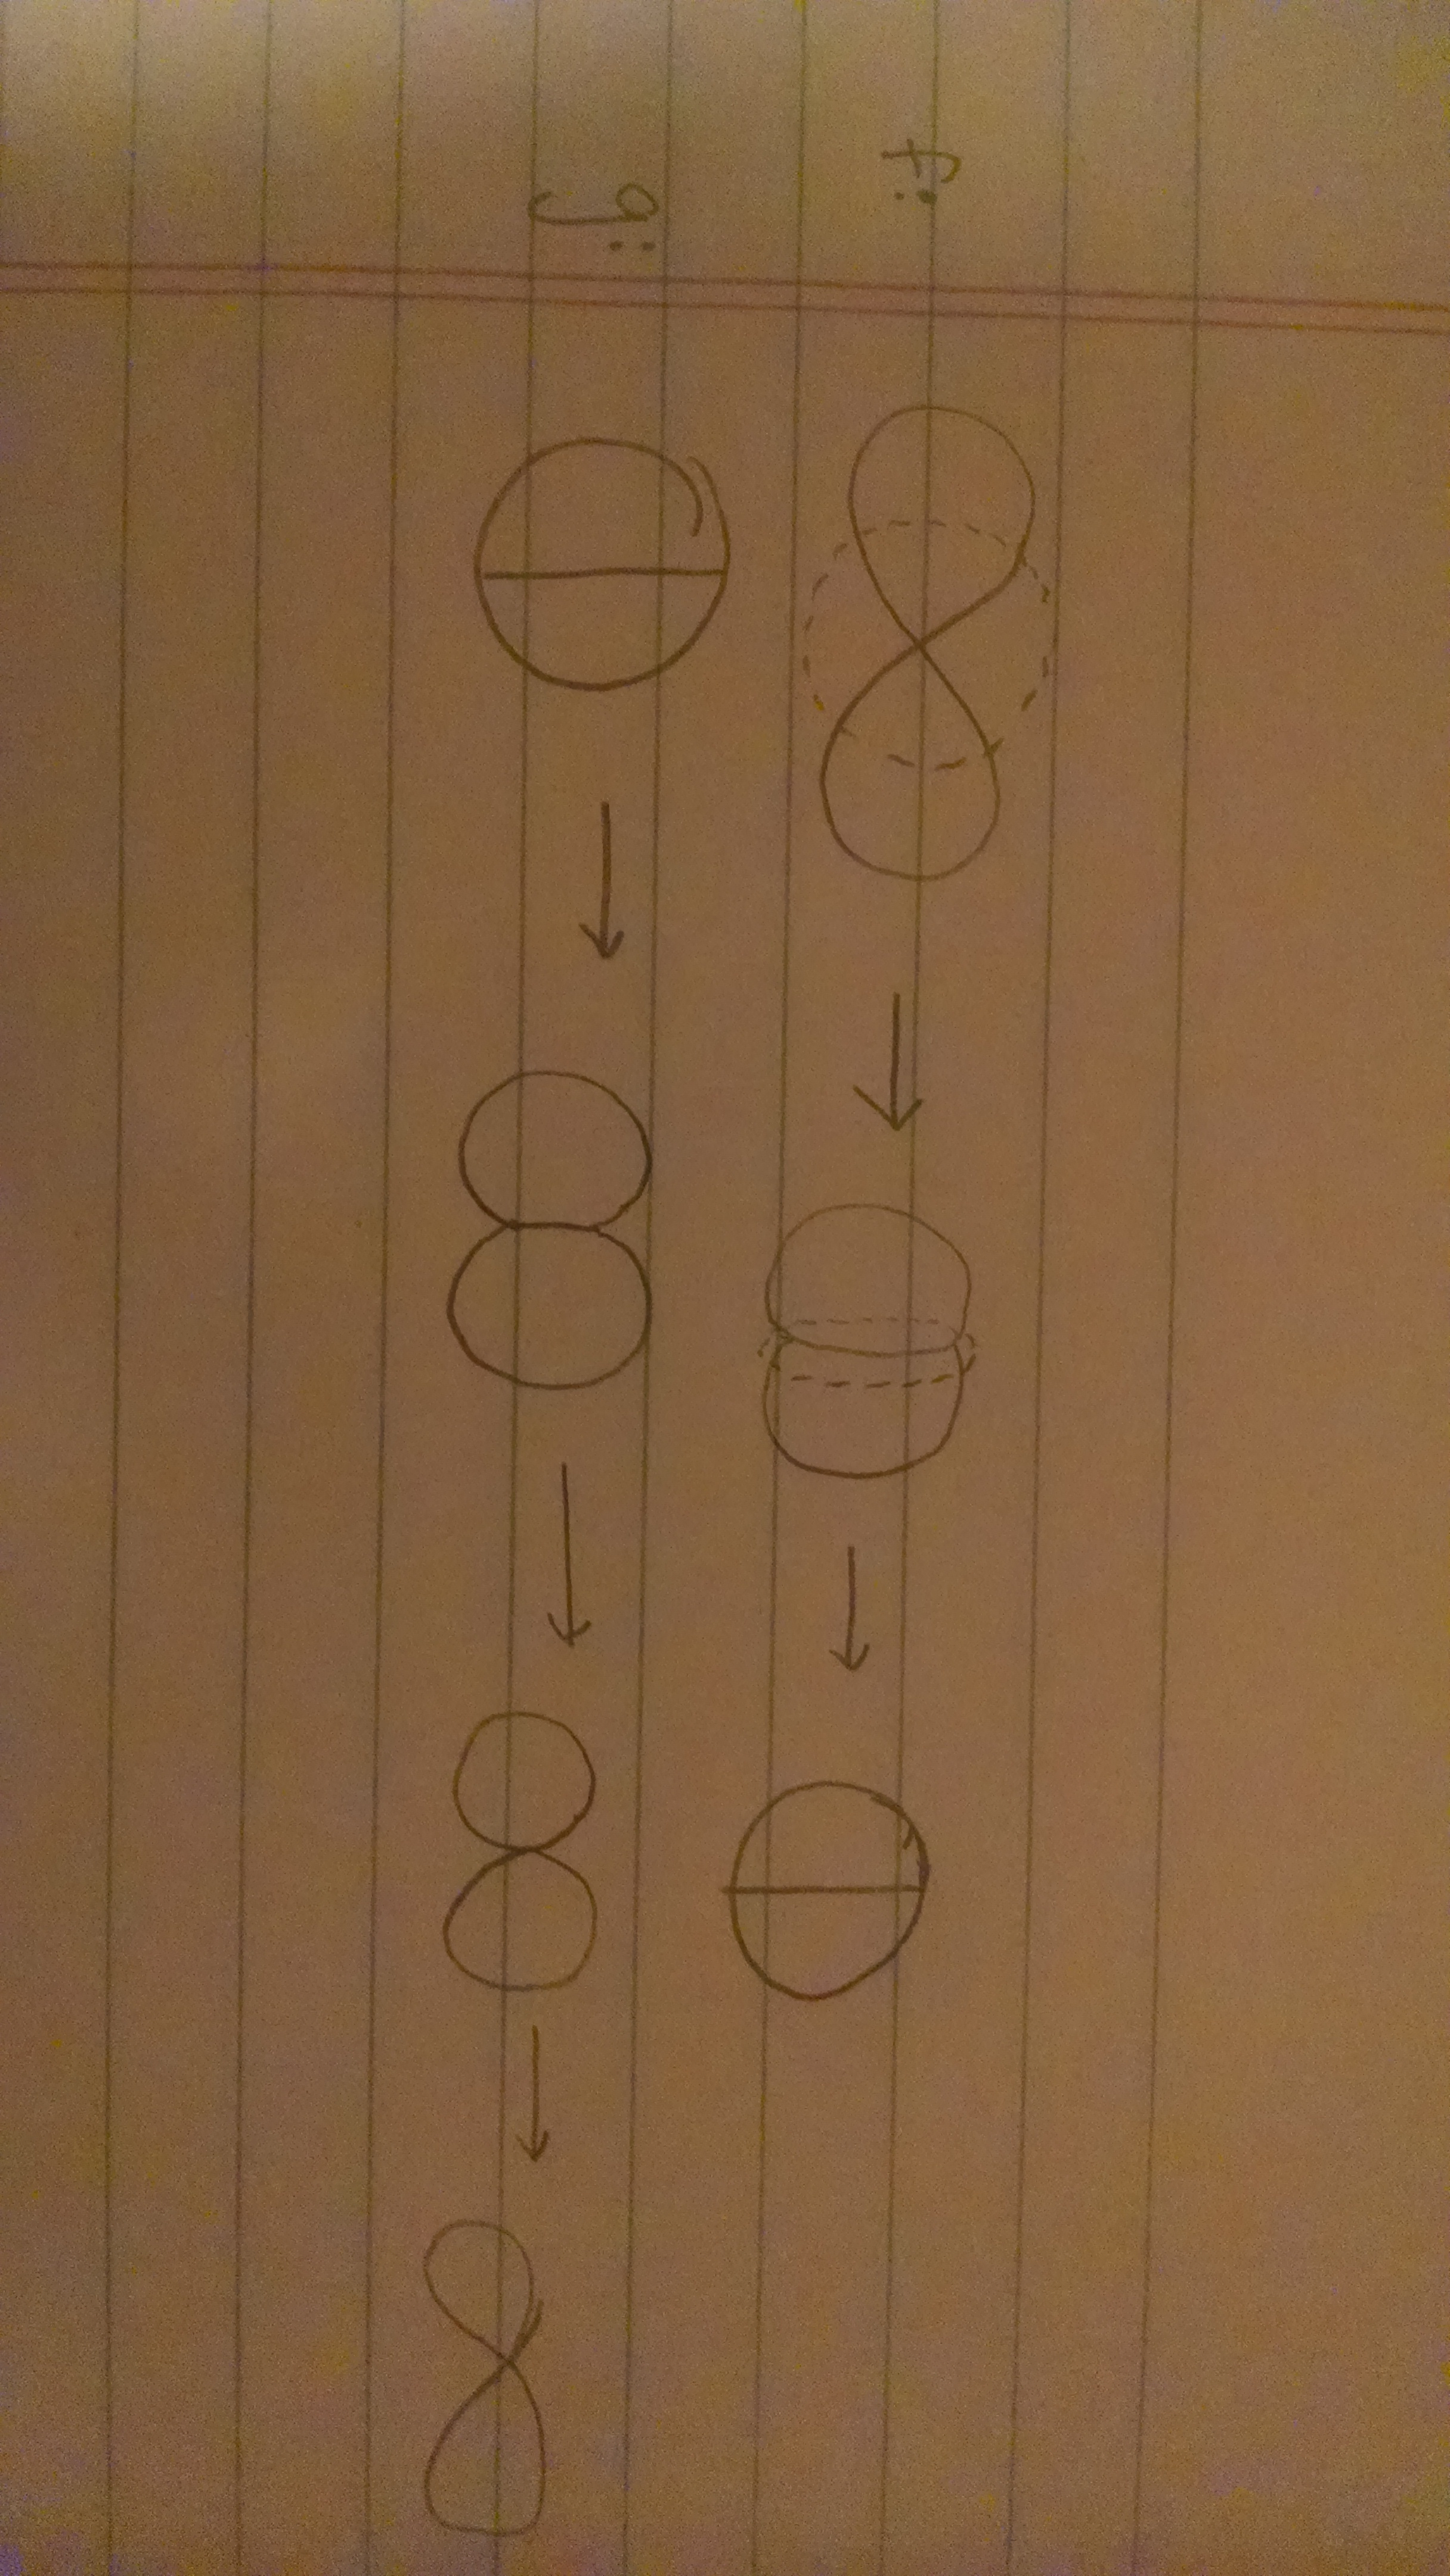
\includegraphics[scale=0.05, angle=90]{inverses.jpg}
\caption{Homotopy inverses between the figure eight and the theta space.}
\label{fig:inverses}
\end{figure}
\end{answer}

\begin{answer}[Page 366, \#10]
Suppose we have assigned an integer for every map $h: S^n \to S^n$ called the degree of $h$ such that:
\begin{itemize}
\item Homotopic maps have the same degree.
\item The deg($h \circ k$) = def($h$) $\cdot$ def($k$)
\item The identity map has degree $1$ and the constant map has degree $0$, and the reflection map $\rho(x_1, \cdots, x_n, x_{n+1}) = (x_1, \cdots, x_n, -x_{n+1}$ has degree $-1$.
\end{itemize}
Next we show some short properties:
\begin{enumerate}
\item We show that there is no retraction $r: \mathbb{B}^{n+1} \to S^n$.
\begin{proof}
Suppose a retraction exists. Then consider the homotopy defined by the below, for $x \in S^n$:
$$
H(x,t) = r(x,t)
$$
Note that $H$ is continuous. However, we have $H(x,0) = r(x,0)$ which is constant and therefore has degree $0$. However, $H(x,1) = r(x,1)$ is the identity for $S^1$, and therefore has degree $1$. This contradicts the above.
\end{proof}
\item We show that if $h: S^n \to S^n$ has degree different from $(-1)^{n+1}$, then $h$ has a fixed point.
\begin{proof}
Following the hint, we first show that if $h$ does not have a fixed point, then $h$ is homotopic to the antipodal map $a(x) = -x$. In fact, the homotopy is given by the following $H: S^n \times I \to S^n$:
$$
H(x,t) = \frac{(1-t)h(x) + ta(x)}{\|(1-t)h(x) + ta(x)\|}
$$
which is valid because $\| (1-t)h(x) + ta(x) \| = 0 \iff (1-t)h(x) = tx \iff t = \frac{1}{2}, h(x) = x$, contradicting the fact that $h$ has no fixed points. Therefore, $h$ is homotopic to the antipodal map $a(x)$. Then note that $a(x)$ has degree $(-1)^{n+1}$ (composition of $n+1$ reflections per coordinate), and by the homotopy above, this implies that $h$ also has degree $(-1)^{n+1}$. Therefore, if $h$ does not have a fixed point, it's degree is $(-1)^{n+1}$. Taking the contrapositive, we the degree is not $(-1)^{n+1}$, then $h$ must have a fixed point.
\end{proof}
\item Next, we show that if $h$ has degree different from $1$, then $h$ maps some point $x$ to its antipode. We prove by contrapositive.
\begin{proof}
Suppose $h$ does not map any points to their antipode $h(x) \neq -x$ for all $x \in S^n$. Then $h$ has degree $1$ because it is homotopic to the identity map. Take the following homotopy:
$$
H(x,t) =  \frac{(1-t)h(x) + tx}{\|(1-t)h(x) + tx\|}
$$
Note that the above is continuous, and we know that $\|(1-t)h(x) + tx\| = 0 \iff (1-t)h(x) + tx  \iff (1-t)h(x) = -tx \iff t = \frac{1}{2}, h(x) = -x$, contradicting our assumption. Therefore $H$ is a valid homotopy with $H(x,0) = h(x)$ and $H(x,1) = x$. Therefore, the degree of $h$ is $1$.
\end{proof}
\item Next, we show that if $S^n$ has a non-vanishing tangent field $v$, then $n$ is odd.
\begin{proof}
Following the hint, we show that if $v$ exists, the identity map is homotopic to the antipodal map. Consider the function $h: S^1 \to S^1$ defined by:
$$
h(x) = \frac{v(x)}{\| v(x)\|}
$$
Then we know that $h(x) = x \iff \langle h(x), x \rangle \neq 0$. However, note that because $v$ is a tangent field, then $\langle h(x), x \rangle = 0$, therefore there exist no point where $h(x) = x$. Similarly, there exists no point where $h(x) = -x$. By the above, since $h$ does not have a fixed point nor does it map a point to its antipode, it must be homotopic to the identity and antipodal maps. Therefore, by the properties given, the degrees of the two maps must be equal. We therefore have that $1 = (-1)^{n+1}$, which implies that $n$ is odd.
\end{proof}
\end{enumerate}
\end{answer}

\begin{answer}[Page 370, \#1]
Suppose $X$ is the union of two copies of $S^2$ having a single point in common. We show that the fundamental group is the trivial group by showing that $X$ is simply connected.
\begin{proof}
We will use Corollary 59.2 and show that $X = U \cup V$, with $U,V$ open and simply connected, and $U \cap V$ non-empty and path connected, which implies that $X$ is simply connected. Let $U = X \setminus \{a\}$ and $V = X \setminus \{b\}$ where $a,b$ come from different distinct copies of $S^2$. Note that $U$ and $B$ are open in $X$. Furthermore, recall that $S^2$ with a point removed is homomorphic to the plane. Then we can construct two reformation retractions $r_1: X\setminus\{a\} \to S^2$ and $r_2: X \setminus \{b\} \to S^2$. The retraction consists of taking the copy from which the point $a$ or $b$ has been removed, and retracting it to the single point of intersection (because it is homeomorphic to $\mathbb{R}^2$). Therefore, it is the case that both $U,V$ are simply connected. Lastly, note that $U \cap V$ is non-empty and that it is path connected because it is homeomorphic to two copies of $\mathbb{R}^2$ joined together at one point. Therefore, the requirements for Corollary 59.2 are satisfied and it is the case that $X$ must be simply connected.
\end{proof}
\end{answer}
\end{document}